%%%%%%%%%%%%%%%%%%%%%%%%%%%%%%%%%%%%%%%%%%%%%%%%%%%%%%%%%%%%%%%%%%%%%%%%%%%%%
%%%% Preamble
%%%%%%%%%%%%%%%%%%%%%%%%%%%%%%%%%%%%%%%%%%%%%%%%%%%%%%%%%%%%%%%%%%%%%%%%%%%%%

%%%% The uwthesis.sty file relies on the memoir class!
%%%% You should be using the memoir class anyway; it makes life easier:
%%%% http://www.ctan.org/tex-archive/macros/latex/contrib/memoir/
\documentclass[oneside, letterpaper, 12pt, oldfontcommands]{memoir}

%%%% Import uwthesis.sty to get official formatting, then set your variables.
\usepackage{uwthesis}
\usepackage{hyperref}
\usepackage{cite}
\usepackage{graphicx}
\newcommand{\fbinv}{\ensuremath{fb^{-1}}}

\newcommand{\PZ}{\ensuremath{Z}}
\newcommand{\Pgamma}{\ensuremath{\gamma}}
\newcommand{\Pn}{\ensuremath{\nu}}
\newcommand{\Pan}{\ensuremath{\bar{\Pn}}}
\newcommand{\zinvg}{\ensuremath{\PZ(\Pn\Pan)\Pgamma}}

\newcommand{\PW}{\ensuremath{W}}
\newcommand{\PWplus}{\ensuremath{W^\mathrm{+}}}
\newcommand{\PWminus}{\ensuremath{W^\mathrm{-}}}
\newcommand{\PWone}{\ensuremath{W^{1}}}
\newcommand{\PWtwo}{\ensuremath{W^{2}}}
\newcommand{\PWthree}{\ensuremath{W^{3}}}
\newcommand{\PB}{\ensuremath{B}}
\newcommand{\Pg}{\ensuremath{g}}
\newcommand{\PH}{\ensuremath{H}}
\newcommand{\Pp}{\ensuremath{p}}
\newcommand{\Pq}{\ensuremath{q}}
\newcommand{\Paq}{\ensuremath{\bar{q}}}
\newcommand{\Pu}{\ensuremath{u}}
\newcommand{\Pd}{\ensuremath{d}}
\newcommand{\Pc}{\ensuremath{c}}
\newcommand{\Ps}{\ensuremath{s}}
\newcommand{\Pt}{\ensuremath{t}}
\newcommand{\Pb}{\ensuremath{b}}
\newcommand{\Pe}{\ensuremath{e}}
\newcommand{\Pmu}{\ensuremath{\mu}}
\newcommand{\Ptau}{\ensuremath{\tau}}
\newcommand{\Pne}{\ensuremath{\Pn_\mathrm{e}}}
\newcommand{\Pnmu}{\ensuremath{\Pn_\mathrm{\mu}}}
\newcommand{\Pntau}{\ensuremath{\Pn_\mathrm{\tau}}}

\newcommand{\pT}{\ensuremath{p_\mathrm{T}}}
\newcommand{\vecpT}{\ensuremath{\vec{p}_\mathrm{T}}}
\newcommand{\ET}{\ensuremath{E_\mathrm{T}}}
\newcommand{\ETgamma}{\ensuremath{E_\mathrm{T}^{\gamma}}}
\newcommand{\MT}{\ensuremath{M_\mathrm{T}}}
\newcommand{\MET}{\ensuremath{p_\mathrm{T}^\mathrm{miss}}}
\newcommand{\vecMET}{\ensuremath{\vec{p}_\mathrm{T}^\mathrm{miss}}}

% Hyphenation of uncommon terms
\hyphenation{cal-ori-me-ter}
\hyphenation{cal-ori-me-ters}

\settitle{A Measurement of \zinvg\ Production and a Search for New Physics in
Monophoton Events Using the CMS Detector at the LHC}
\setauthor{James Joseph Buchanan}
\setdepartment{Physics}
\doctors % or \masters
\setgraddate{2018}
\setdefensedate{T.B.D.} % or whatever format you want

%%%% Members of the Final Oral Committee (FOC)
%%%% Give name, rank, and department
%%%% 
\setfoca{Sridhara Dasu}{Professor}{Physics} % <- Your advisor
\setfocb{Wesley Smith}{Emeritus Professor}{Physics}
\setfocc{Matt Herndon}{Professor}{Physics}
\setfocd{T.B.D.}{Professor}{Physics}
\setfoce{T.B.D.}{Professor}{Something Else}
% \setfocf{Grover Cleveland}{Professor}{Zoology}

%%%% Your abstract, used for the UMI abstract and in your front matter
\setabstract{%
  This thesis presents several studies of monophoton final states
  using 35.9 $fb^{-1}$ of 13 TeV proton-proton collision data collected by the CMS
  experiment at the LHC in 2016. The standard model \zinvg\ cross section is measured
  as a function of photon transverse momentum. No significant deviations from standard
  model predictions are observed.
  The results are also interpreted in the context of several new physics models.
  Limits are placed on coupling strengths of anomalous triple gauge couplings between
  photons and \PZ\ bosons,
  new particle masses in simplified models of dark matter, the suppression scale of a dark matter
  effective field theory model, and the graviton mass scale in a model of extra
  spatial dimensions.
}

%%%%%%%%%%%%%%%%%%%%%%%%%%%%%%%%%%%%%%%%%%%%%%%%%%%%%%%%%%%%%%%%%%%%%%%%%%%%%
%%%% Document
%%%%%%%%%%%%%%%%%%%%%%%%%%%%%%%%%%%%%%%%%%%%%%%%%%%%%%%%%%%%%%%%%%%%%%%%%%%%%

\begin{document}

% Tell the memoir class to set up lowercase roman for pagination, etc.
\frontmatter

%%%% Uncomment this to create a UMI abstract page.
%%%% If you are submitting electronically, however, this page is unnecessary.
% \theumiabstract

% The title page
\thetitlepage
\clearpage

% The copyright page, if you want to pay the fee and register copyright.
\thecopyrightpage
\cleardoublepage

% These above pages should not be counted, so we reset the counter to 1.
\setcounter{page}{1}

% An abstract may be required by your department.
\section{Abstract}
\uwabstract
\cleardoublepage

% Acknowledgements go here if you want to include them.
\section{Acknowledgements}
Acknowledgements go here.
% These results would never have come to fruition without the support of my colleagues
% and friends in the UW-Madison CMS group.
% Wesley Smith, Sridhara Dasu, and Matt Herndon are great physicists and leaders
% who have nurtured a rigorous standard of excellence that this group
% can rightly be proud of.
% Bhawna Gomber's deep expertise, organizational acumen,
% and untiring work ethic have pushed these analyses forward at every step. These
% results are as much hers as they are mine.
% Tom Perry developed a previous iteration of these analyses,
% and freely contributed his assistance and code to let us hit the ground running in 2016.
% Devin Taylor, Tyler Ruggles, Nate Woods, Laura Dodd, Nick Smith, Kenneth Long, and
% Usama Hussein were all excellent office mates, always available to lend
% their considerable knowledge and insight at the drop of a hat, a privilege I have taken advantage
% of on innumerable occasions.
% I must finally thank my parents, Yvonne and Darryl Buchanan,
% for their perpetual support of everything I do.
\clearpage

% Table of contents
\maxtocdepth{subsection}
\tableofcontents* % the * means that there isn't an entry for the TOC itself
\clearpage
\listoffigures  % if you have any figures
% \clearpage
% \listoftables   % if you have any tables

% Tell the memoir class to set up normal pagination, etc. for the main doc
\mainmatter

\chapter{Introduction} \label{sec:introduction}
\section{Overview} \label{sec:introduction_overview}
This thesis presents several analyses of event
yields in ``monophoton'' final states, characterized by a single \Pgamma\ with high transverse
momentum, along with an overall transverse momentum imbalance typically of equal magnitude and opposite direction to
that of the photon.
These analyses correspond to 35.9 \fbinv\ of 13 TeV proton-proton (\Pp\Pp) collision data collected in 2016 by the CMS
detector at the LHC. A measurement of the production rate for the process $\Pp\Pp \to \PZ\Pgamma \to \Pn\Pan\Pgamma$ is obtained
and compared to predictions derived from the standard model (SM) of particle physics. No significant deviation from SM
predictions is observed.

The predicted monophoton yield in several theories of physics beyond the SM (BSM) is higher than the SM prediction.
This thesis examines two varieties of anomalous triple gauge coupling (aTGC), simplified models of dark matter (DM)
interacting with SM matter via a vector or axial-vector mediator, an effective field theory (EFT) of DM interaction
with  \Pgamma\ and \PZ\ bosons, and a model of extra spatial dimensions. For each of these models, 95\% confidence level (CL)
limits are placed on relevant parameters based on the observed collision data.

\section{Standard model of particle physics} \label{sec:introduction_standard_model}
The ``standard model'' of particle physics is our current best mathematical framework for describing the behavior
of elementary particles. The set of particles described by the SM is illustrated in Fig.~\ref{fig:sm_particles}, which
groups them according to certain fundamental characteristics.
Each particle has an intrinsic angular momentum known as spin, specified by the lower number in each square of Fig.~\ref{fig:sm_particles}.
Spin can be an integer or half-integer, according to which the particle is classified as a boson or fermion, respectively.
The fundamental fermions comprise six ``flavors'' of quarks and six flavors of leptons,
each of which has both a particle and an anti-particle variety; the quarks additionally come in three ``colors''.
We denote a particle by a letter, e.g. $q$ for a generic quark, and its antiparticle partner by an overbar, e.g. $\bar{q}$.
The fundamental bosons comprise the scalar \PH\ as well as the gauge bosons, in turn comprising the \PZ, photon (\Pgamma),
two \PW s distinguished by their electric charge, and eight gluons (\Pg) distinguished by a doublet of colors.

\begin{figure}[hbtp]
  \begin{center}
    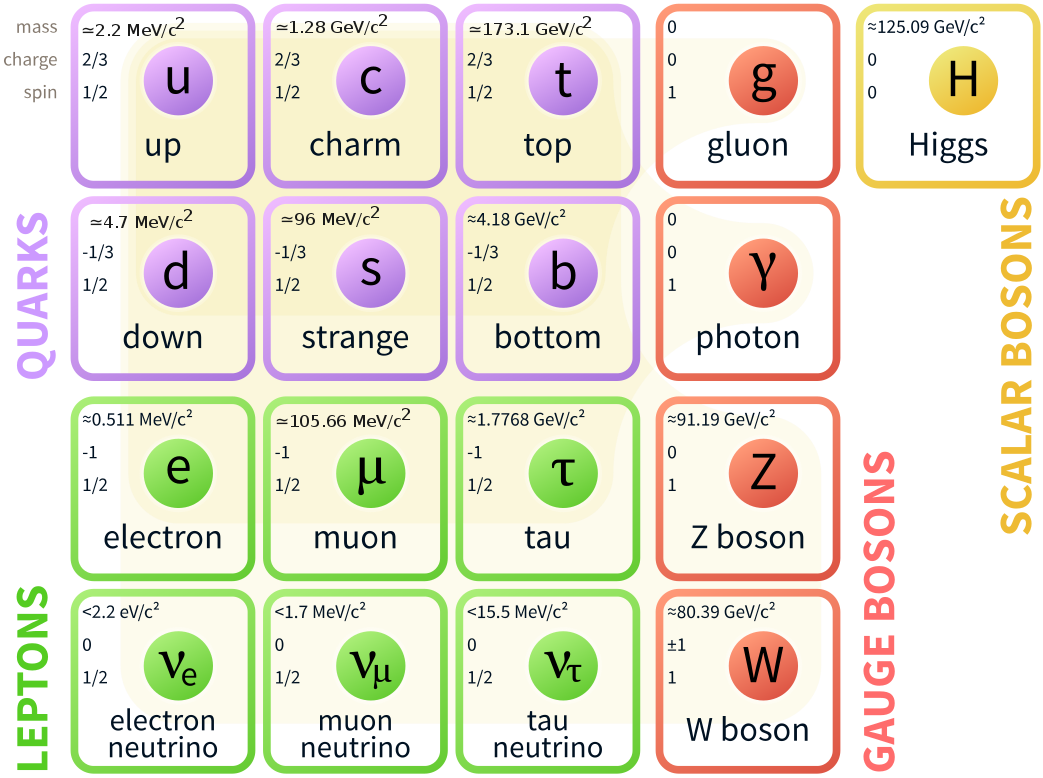
\includegraphics[width=1.0\textwidth]{Figures/sm_particles.png}
    \caption{
      The particles of the Standard Model.
    }
    \label{fig:sm_particles}
  \end{center}
\end{figure}

The particles are related to one another through various
classes of interactions, each of which has a corresponding charge whose sum must be conserved in any physical process.
The electromagnetic and weak interactions correspond to electric charge and weak isospin, respectively.
In Fig.~\ref{fig:sm_particles}, the electric charge is specified by the middle number in each square.
For quarks and leptons, weak isospin determines whether the particle is ``up-type''
(\Pu, \Pd, \Pt, \Pne, \Pnmu, \Pntau) or ``down-type'' (\Pd, \Ps, \Pb, \Pe, \Pmu, \Ptau).
The \PH\ has a down-type weak isospin, the two \PW\ bosons each have a weak isospin matching their electric charge
(but with twice the magnitude of that of the fermions), and the other bosons have none.
By virtue of the \PH, the electromagnetic and weak interactions are intermingled into what
is called the electroweak (EWK) interaction.
The three colors carried by quarks and gluons are associated with an interaction described by the theory of quantum
chromodynamics (QCD). The preceding discussion applies to normal (i.e. not anti-) particles; antiparticles carry opposite values of all the
aforementioned charges.

These interactions lead to the relationships illustrated in Fig.~\ref{fig:sm_interactions}, in which every linkage represents
a direct ``coupling'', which allows a particle at one end of the link to evolve directly into a particle at the other end.
Particles with a nonzero electric charge are all coupled directly to the photon. The photon is coupled to the weak bosons
(\PZ\ and \PW), which in turn couple to all of the fundamental fermions.
The gluons couple directly with each other and with the quarks.
Particles that couple directly to the \PH\ have an intrinsic mass (specified by the top number in each square of Fig.~\ref{fig:sm_particles})
tied to the strength of their coupling. In the SM, any particle that does not couple directly to the \PH\ is massless.
The SM has been profoundly well-studied and is extremely successful in its predictive capacity, as documented in numerous comprehensive
texts on the subject, e.g.~\cite{ref:HalzenMartin, ref:PDG}.

\begin{figure}[hbtp]
  \begin{center}
    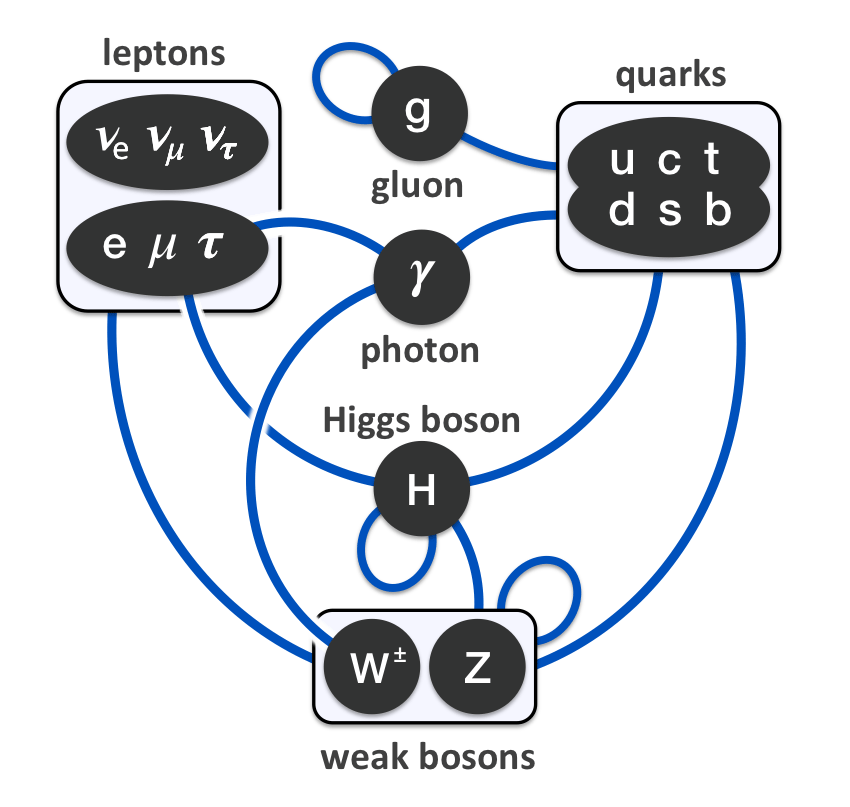
\includegraphics[width=0.7\textwidth]{Figures/Elementary_particle_interactions_in_the_Standard_Model.png}
    \caption{
      Standard Model couplings.
    }
    \label{fig:sm_interactions}
  \end{center}
\end{figure}

\section{\textorpdfstring{\zinvg}{Z(νν)γ} cross section} \label{sec:introduction_znng}
Specific processes of particle evolution can be illustrated using Feynman diagrams. These are
assembled by combining fundamental interaction vertices: the SM vertices relating the fermions and gauge bosons are listed in Fig.~\ref{fig:sm_vertices}.
A diagram without internal loops is called a tree-level diagram. A diagram with a loop has at least one more vertex than that same
diagram with the loop removed, and the more vertices a diagram has, the less it tends to contribute to the expected yield for a
given process. Hence, the simplest tree-level diagrams for a process are the most dominant in their effects.

\begin{figure}[hbtp]
  \begin{center}
    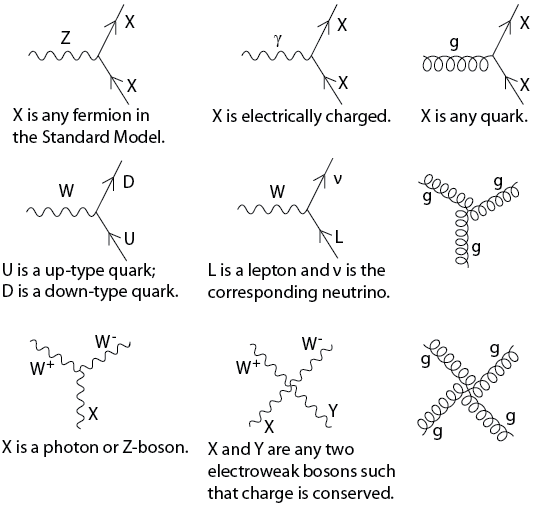
\includegraphics[width=0.7\textwidth]{Figures/Standard_Model_Feynman_Diagram_Vertices.png}
    \caption{
      Fermion and gauge boson vertices of the standard model.
    }
    \label{fig:sm_vertices}
  \end{center}
\end{figure}

In the SM, events with a monophoton signature arise at the LHC (chapter ??) primarily from the process $q\bar{q} \to \PZ\Pgamma \to \Pn\Pan\Pgamma$,
where $q$ is any single species of quark, \Pn\ is any single species of neutrino, and the neutrino-antineutrino pair arises from the decay
of a short-lived \PZ\ boson. The leading tree-level diagram for this process is shown in Fig.??. We typically abbreviate this process by
reference to its final state, \zinvg.



\section{Anomalous triple gauge couplings} \label{sec:introduction_aTGC}
Putative vertices joining three particles that are not found in the SM are known as aTGCs. For example, there is no fundamental SM vertex
joining a single \Pgamma\ to a pair of \PZ s, or a single \PZ\ to a pair of \Pgamma s. A model
describing the generic phenomenology of these aTGCs is developed in~\cite{ref:Nucl.Phys.0550-3213_87_90685-7, ref:PhysRevD.47.4889, ref:PhysRevD.62.113011}.
For an intermediate state $V = \PZ,\Pgamma$ decaying to a final state \PZ\Pgamma\ pair, this model parametrizes the effective vertex interaction $\PZ\Pgamma V$
by a set of factors $h_{i}^{V}$ ($i$ from 1 to 4). Increasing the values of these parameters significantly increases the predicted rate of occurrence
of \zinvg\ processes, by allowing the reaction to proceed via the diagram shown in Fig.??, in which the aTGC vertex is covered by an opaque circle.

The circle could be thought of as masking a more detailed process taking place underneath. The SM admits processes that are predicted to contribute
to this effective vertex, but all SM contributions to $h_{3,4}^{V}$ have at least one internal loop that could fit within the circle, and
further loops are required for $h_{1,2}^{V}$ contributions~\cite{ref:PhysRevD.47.4889}.
As a consequence, the SM contribution to all eight $h_{i}^{V}$ parameters is quite close to zero.
The observation of a substantial nonzero value for any $h_{i}^{V}$ would be a compelling sign of BSM physics.

The contributions to the \zinvg\ production rate coming from $h_{1,2}^{V}$ are independent of those from $h_{3,4}^{V}$ (for any V), and also nearly identical
in magnitude, so without loss of generality we only focus on scenarios for which $h_{3,4}^{V}$ are nonzero. The contributions
from $h_{i}^{\PZ}$ are largely independent of those from $h_{j}^{\Pgamma}$ (for any i,j), so these are examined separately.
However, the contributions from $h_{3}^{V}$ are substantially correlated with those from $h_{4}^{V}$ (and similarly for $h_{1,2}^{V}$), so we examine
scenarios in which $h_{3,4}^{V}$ take on assorted pairs of values, both of which may be nonzero. The theoretical relationships between these parameters
are explored in~\cite{ref:PhysRevD.47.4889}.

\subsection{Previous searches} \label{sec:introduction_aTGC_previous_searches}
The LEP collider established constraints on each of the eight the parameters $h_{i}^{V}$ in the context of the process $e^{\mathrm{+}}e^{\mathrm{-}} \to \PZ\Pgamma$.
In a statistical combination of searches perfomed by the DELPHI, L3, and OPAL experiments, examining 3 $fb^{-1}$ of $e^{\mathrm{+}}e^{\mathrm{-}}$ collision data
at center-of-mass energies ranging from 130 GeV to 209 GeV, the 95\% CL intervals of seven of the parameters contain 0, with total ranges between 0.05 and 0.10 for $h_{i}^{\Pgamma}$
and between 0.14 and 0.25 for $h_{i}^{\PZ}$; the 95\% CL interval for the remaining factor $h_{4}^{\gamma}$ spans 0.01 to 0.05~\cite{ref:j.physrep.2013.07.004}.

The LEP combined analysis assumed that all but one of the eight parameters were fixed to the SM expectation of 0.
It was also the last major effort to obtain limits on $h_{1,2}^{V}$ independently of $h_{3,4}^{V}$,
as subsequent searches have taken the present approach of focusing on $h_{3,4}^{V}$ alone, for the reasons listed above.
Uniquely among the LEP experiments, the L3 Collaboration also placed limits on correlated pairs of parameters, shown in Fig.~\ref{fig:L3_atgc_contours}~\cite{ref:j.physletb.2004.07.002}.

\begin{figure}[hbtp]
  \begin{center}
    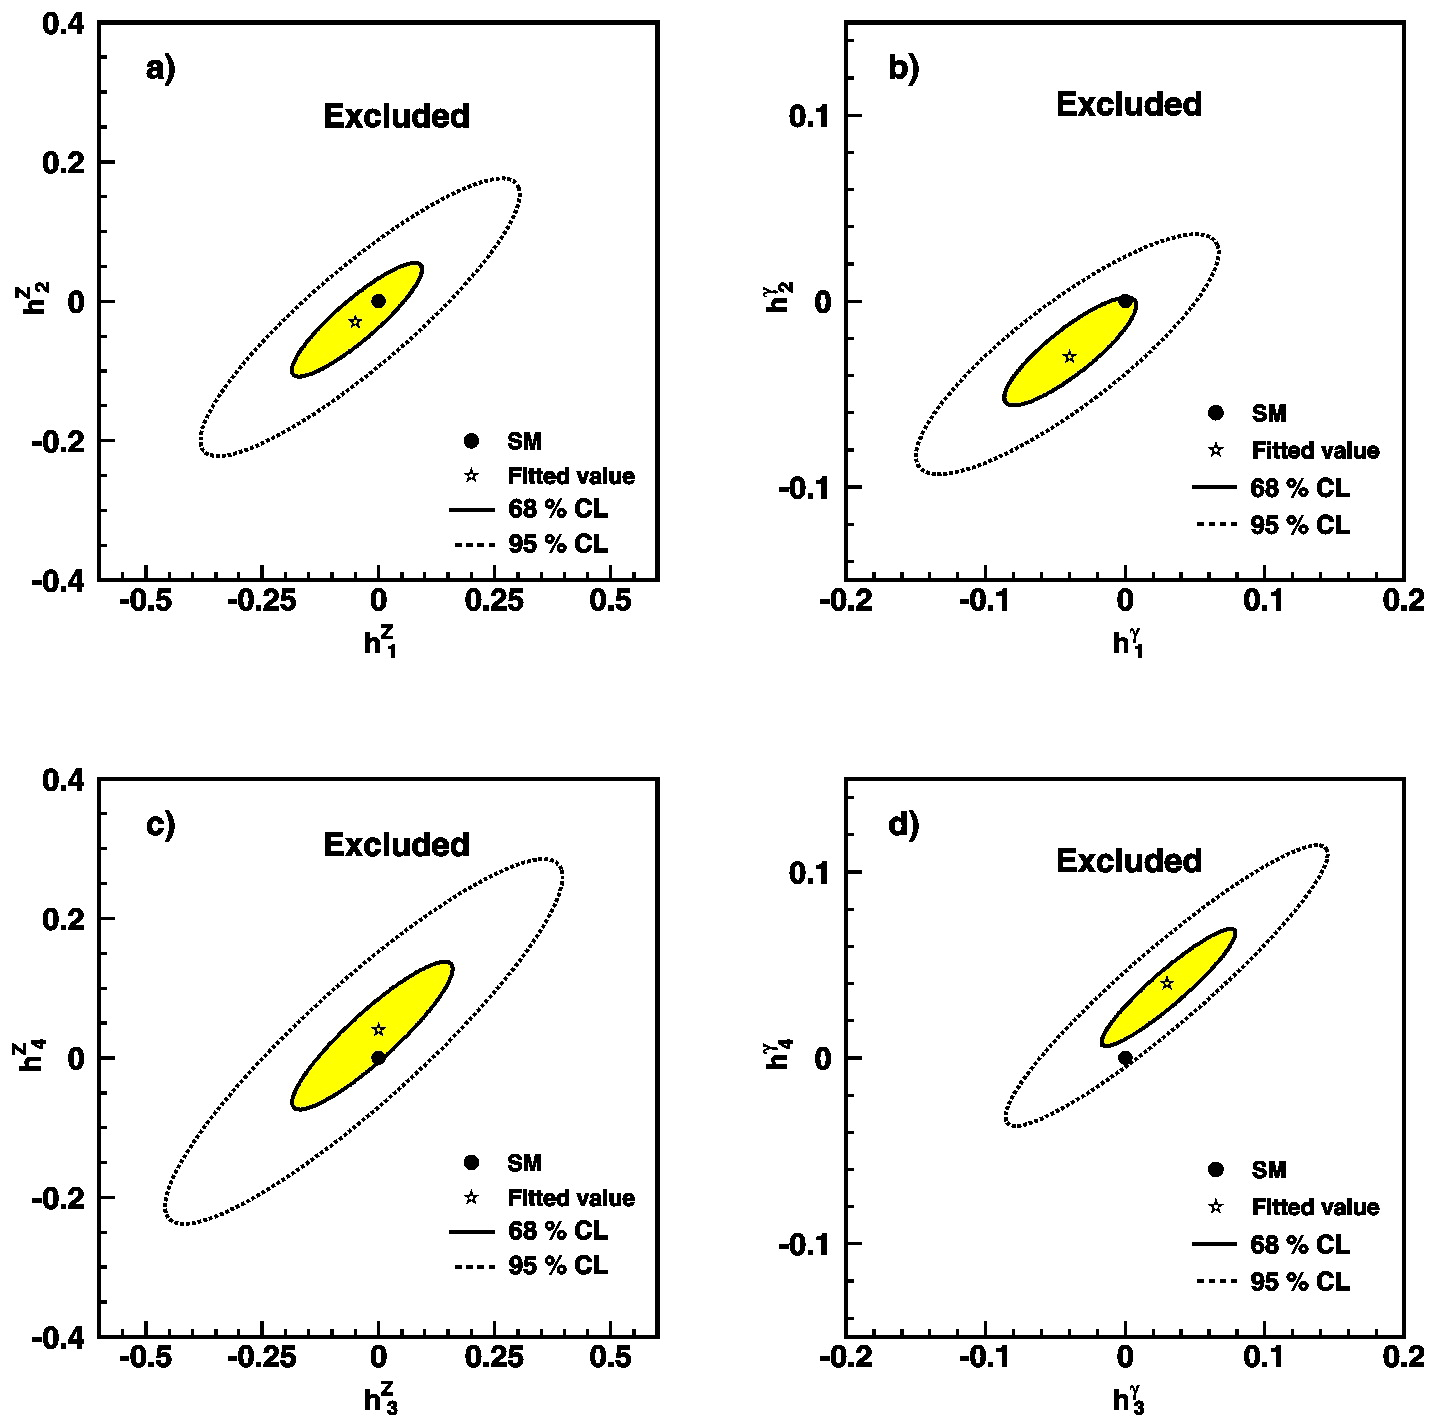
\includegraphics[width=0.7\textwidth]{Figures/L3_atgc_contours.jpg}
    \caption{
      $h_{i}^{V}$ exclusion contours from the L3 experiment at the LEP collider~\cite{ref:j.physletb.2004.07.002}.
    }
    \label{fig:L3_atgc_contours}
  \end{center}
\end{figure}

This form factor was introduced in the common reference~\cite{ref:PhysRevD.47.4889} but was not used in LEP~\cite{ref:j.physrep.2013.07.004}
or subsequent LHC analyses, which treat the $h_{i}^{V}$ parameters as constants.

None of these analyses report any significant deviation from SM predictions.

\section{Dark matter simplified models} \label{sec:introduction_dark_matter}
The SM does not explain every observed natural phenomenon. One example of a phenomenon with no apparent SM explanation is so-called ``dark matter''.
On cosmological scales there appears to be an abundance of massive
matter with no interactions of any sort other than its gravitational pull. No SM particle is predicted to exhibit this behavior, and
this has spurred the development of BSM theories aiming to account for it.

The circle obscuring the DM vertex
denotes that this is an effective vertex in the generic model that mimics the behavior of true vertices in a full theory of particle physics,
such as the SM. Like the ADD theory discussed in Sec.~\ref{sec:introduction_ADD}, this model is only capable of making meaningful physical
predictions within a restricted kinematic range. These theories are meant to encapsulate highly generic, model-independent features of potential
new-physics phenomena, but outside of their range of kinematic validity, the fully generic description must break down as more specific,
model-dependent BSM signatures manifest themselves.

\section{ADD gravitons} \label{sec:introduction_ADD}

\bibliographystyle{utcaps}
\bibliography{references}
\end{document}
